\documentclass[11pt]{article}

\usepackage[margin=1in]{geometry}
\usepackage{amsmath}
\usepackage{amssymb}
\usepackage{booktabs}
\usepackage{array}
\usepackage{graphicx}
\usepackage[hidelinks]{hyperref}
\usepackage{xcolor}

% Placeholder box for figures whose source data lives on the Windows machine
% or which haven't been generated yet. Renders a visible bordered box with
% a label so the reader can see exactly where the figure goes.
\newcommand{\figplaceholder}[2]{%
  \fbox{\parbox{0.9\linewidth}{\centering
    \vspace{2.2cm}
    \textbf{[FIGURE PLACEHOLDER: \texttt{#1}]}\\[2pt]
    \textcolor{gray!70}{Data source: \texttt{#2}}\\
    \vspace{2.2cm}
  }}%
}

\title{Cryptocurrency pair spreads:\\
a screening-artifact audit and the marginal survivor}
\author{Jack Lutz \and Sammy Adham \and Frank Kronewitter}
\date{\today\\[0.4em]\small Advisor: Mihai Cucuringu}

\begin{document}

\maketitle

\begin{abstract}
We set out to build a profitable statistical arbitrage strategy on hourly cryptocurrency
pair spreads. It did not work, and this paper is mostly about why.
Two screens that appear to find strong, tradable structure fail matched placebos in a way most consistent with their being statistical artifacts. A
Kalman dynamic hedge ratio appears to produce stationary, mean-reverting spreads for nearly
the entire liquid universe, but it runs a stationarity test on a filter's own innovations,
which are white by construction. Placebos that cannot be cointegrated pass the same screen at
the same nearly $100\%$ rate, while a clean test finds genuine out-of-sample cointegration in
only a few percent of pairs. A rolling $z$ score appears to generate a large reversion edge,
but it reverts mechanically even on a pure random walk. Both artifacts hold at hourly,
four-hour, and daily frequencies. Once we benchmark against placebos, the structure that
survives is either priced too fast to trade or too marginal to deploy. Order flow information in
the Level 2 book decays within seconds. Reversion speed ranks pairs (Spearman $\rho = 0.46$), but
the ranking does not turn into profit. The one market-neutral mean-reversion book that clears
honest accounting posts a HAC- and venue-adjusted monthly Sharpe near $1.0$,\footnote{All Sharpe
figures in this paper are unit-notional and capacity-unbounded; impact is not modeled. See
Limitations.} and only without a stop and only as a multiweek hold. That $1.0$ is an
exploratory, post-hoc estimate that was never preregistered, and our preregistered test gives a
confidence interval spanning zero, so we claim no significant tradable edge. We read this as evidence that the
liquid core of crypto pair spreads is efficient.
\end{abstract}

% =====================================================================
\section{Introduction}
\label{sec:intro}

The goal at the outset was a profitable hourly pairs strategy on crypto. We did not get one, and
the useful finding is why: the two screens that made the strategy look best are statistical
artifacts, and whatever structure is genuinely present is either priced within seconds or too thin
to trade once costs and selection are counted.

The project began in the pairs trading tradition of Gatev, Goetzmann, and
Rouwenhorst~\cite{gatev2006pairs}: find two assets whose prices hold a stable relationship, trade the
spread when it deviates, and collect the reversion. Cryptocurrency is a natural place to look,
with a continuously traded market and a rapidly changing set of listed coins. Our proposal was noncommittal about profit from the start. It framed the goal as quantifying whether stable mean-reverting
relationships exist in crypto, ``as a way of gaining a deeper understanding of market efficiency
and information flow.'' This paper answers that question, and the answer is mostly negative.

We claim three contributions, each bounded against prior work as cited. The first rests on
empirical demonstration plus a conjectural transfer of the Ero\u{g}lu, Miller, and Yi\u{g}it
mechanism to the frozen-filter innovation sequence; a formal proof at that level is
open. With that caveat: first, two standard pair screening tools manufacture the appearance of
structure on data that cannot carry it. A Kalman dynamic hedge cointegration test passes
random walk, phase-randomized, and block-shuffled placebos at the same near-$100\%$ rate it
passes real pairs, and a positive control of constructed cointegrated pairs passes at the
same rate as the random-walk negative: at the critical values used in this pipeline, the screen
does not separate real pairs from matched placebos. A rolling $z$ score reverts mechanically on pure random walks, producing
per-event reversion of $+0.98z$ to $+1.61z$ across hourly, four-hour, and daily frequencies
and a Sharpe near $2.2$ on random-pair placebos against $4.75$ on the actual data. The
underlying mechanisms are known: a well specified Kalman filter has white steady state
innovations~\cite{harvey1989structural}, rolling mean demeaning induces negative
autocorrelation~\cite{working1960correlation, cochrane1988random}, and Ero\u{g}lu, Miller,
and Yi\u{g}it~\cite{eroglu2022tvc} show that time-varying-parameter Kalman models are
vulnerable to spurious regression because the integrated error is transferred to the
estimated state equation. Our contribution is the screen-level placebo audit: for the
Kalman ADF screen, on the Kalman dynamic hedge plus ADF pipeline that circulates in pairs
trading practice (\cite{vidyamurthy2004pairs, elliott2005pairs,
triantafyllopoulos2011dynamic}), with a positive control showing the screen cannot
separate constructed cointegrated pairs from random walks; and for the rolling $z$ rule,
the random-real-pairs bootstrap of Gatev, Goetzmann, and
Rouwenhorst~\cite{gatev2006pairs} is the closest prior precedent, extended here to
synthetic random-walk and phase-randomized nulls with per-event reversion magnitudes
reported in $z$-units. Second, extending
Schnaubelt's~\cite{schnaubelt2022rl} large-scale RL placement study on crypto L2, we run a
specification-style test on a four-major basket (BTC, ETH, SOL, AVAX) with $29{,}952$ parent
orders on event-level Binance L2 data in 2024. Aggressive crossing is cheapest across all
four symbols, the signal correlates $+0.03$ with the per-order advantage of posting over
crossing, and a perfect foresight oracle bounds achievable savings at $1.4$ bps: the
opportunity exists but no contemporaneous feature realizes it. Third, the candidate market-neutral reversion
strategy that emerges from the surviving structure clears honest accounting at a venue- and
HAC adjusted monthly Sharpe near $1.0$, only without a stop, and a preregistered held-out
backtest of it inflates above the in-sample number on uncostable microcap moves; our one
surviving result ends up cutting against itself.

The backtest-overfitting
literature~\cite{bailey2014dsr} stress tests the strategy you finally pick;
the screen you used to build the spread needs the same scrutiny.

To restate the scope. The Kalman screen
mechanism is from Ero\u{g}lu, Miller, and Yi\u{g}it~\cite{eroglu2022tvc} and our extension is
the screen-level placebo audit and the positive control. The L2 execution test extends
Schnaubelt~\cite{schnaubelt2022rl} with an oracle bound and a null result on a smaller
basket. The survivorship analysis combines point-in-time crypto cross-sections (Ammann,
Burdorf, Liebi, and St\"ockl~\cite{ammann2022survivorship}; Liu, Tsyvinski, and
Wu~\cite{liu2022common}) with a leg-level break-aware stop (Lu and
Lai~\cite{lu2021structural}) and asks the joint question for crypto pair spreads. None of
the three is unconditional novelty; each is a deliberate addition on top of cited prior work.

% =====================================================================
\section{Related work}
\label{sec:related}

Three bodies of prior work set up this paper. The two screens we audit come from the
cointegration branch of the pairs trading literature. The order flow tools we apply to crypto
L2 data are standard market microstructure. And the crypto market efficiency literature is
where our headline negative result has to be read.

\subsection{Pairs trading and dynamic cointegration}
\label{sec:related-pairs}

The cointegration branch of pairs trading descends from Engle and
Granger~\cite{engle1987cointegration}, with its practitioner facing version codified in
Vidyamurthy~\cite{vidyamurthy2004pairs}: fit a spread, test the residual for stationarity,
trade deviations of the residual. The two screens we audit in Section~\ref{sec:artifacts}
are standard implementations of that pipeline. The state space variant comes from Elliott,
van der Hoek, and Malcolm~\cite{elliott2005pairs}, who model the spread as a discrete time
Ornstein-Uhlenbeck process observed in Gaussian noise. Triantafyllopoulos and
Montana~\cite{triantafyllopoulos2011dynamic} extend it to time varying parameters with
online estimation, which is the Kalman dynamic hedge we run. The distance based
alternative of Gatev, Goetzmann, and Rouwenhorst~\cite{gatev2006pairs} is the standard
benchmark.
Harvey's classical state space text~\cite{harvey1989structural} states the steady state
whitening property we exploit. The closest econometric prior is Ero\u{g}lu, Miller, and
Yi\u{g}it~\cite{eroglu2022tvc}, who show that time-varying-parameter Kalman cointegration
models suffer from spurious regression because the integrated error is transferred to the
estimated state equation; they propose corrections at the cointegrating-vector level. Our
paper applies the consequence of that finding at the screen level: the specific
Kalman-plus-ADF pipeline used as a tradability filter cannot discriminate cointegrated
pairs from random walks, and we document this empirically with matched placebos and a
positive control.

\subsection{Microstructure and order flow}
\label{sec:related-micro}

The information content of order flow is the central object of classical microstructure,
beginning with Kyle~\cite{kyle1985continuous} on the linear price impact of informed
trading. Hasbrouck~\cite{hasbrouck1991measuring} introduces the permanent versus transient
decomposition of trade impact, which we use to interpret the seconds-scale half-life we
observe. The event-time order flow imbalance of Cont, Kukanov, and
Stoikov~\cite{contkukanovstoikov2014} predicts sub-second mid moves nearly linearly on
equities; we replicate this on Binance L2 in 2024 for BTC, ETH, SOL, and AVAX. We use the
size-weighted microprice of Stoikov~\cite{stoikov2018microprice} as our regression target.
The toxicity program of Easley, L\'opez de Prado, and O'Hara~\cite{easley2012vpin} is the
natural place to look for a tradable order flow signal at longer horizons, but Andersen and
Bondarenko~\cite{andersen2014vpin} show its predictive content is largely mechanical and
its sign is sensitive to trade classification. Our crypto VPIN measurement replicates their
critique.

\subsection{Cryptocurrency market efficiency}
\label{sec:related-crypto}

The crypto efficiency literature has converged on a picture our results are consistent
with: the most-traded coins on the most-traded venues look weak-form efficient, while
thinner segments do not. Urquhart's~\cite{urquhart2016inefficiency} original Bitcoin tests
rejected EMH on early daily data but already noted the second half of the sample looked
tighter. Wei~\cite{wei2018liquidity} shows on 456 coins that return predictability and
Hurst persistence collapse with liquidity, and Brauneis and Mestel~\cite{brauneis2018price}
replicate the link across 73 coins and eight tests. Makarov and
Schoar~\cite{makarov2020trading} show that persistent cross-exchange price gaps survive
transaction costs and are best explained by capital-control and credit frictions, which
mirrors why our Coinbase adjusted Sharpe sits below the Binance.US figure. The closest
prior on crypto pairs is Fil and Kristoufek~\cite{fil2020pairs}, who find that most
strategies underperform their benchmarks once costs are realistic; our honest accounting
Sharpe of $\sim$$1.0$ is consistent with their picture.

\subsection{Machine learning approaches}
\label{sec:related-ml}

Krauss, Do, and Huck~\cite{krauss2017deep} apply deep neural networks, gradient boosted
trees, and random forests to S\&P~500 statistical arbitrage and find ensemble lifts that
erode sharply after costs. Our XGBoost / LSTM / transformer comparison reproduces the same
pattern on crypto pairs: a calibrated spread $z$ score carries roughly $79\%$ of the P\&L of
a four architecture stack, in line with the multiple testing cautions of L\'opez de
Prado~\cite{lopezdeprado2018advances}. The deep-learning literature on limit order book
data predicts at sub-second horizons, which is shorter than our hourly bars and consistent
with our finding that L2 order flow information decays within $30$ seconds and does not
survive to a tradable horizon.

\subsection{Position relative to prior work}
\label{sec:related-novelty}

Each of this paper's three contributions is bounded against prior art. We list what we add
on top of the cited literature, not what is unconditionally new. First, the screen-level
placebo audit of the Kalman dynamic hedge plus ADF cointegration pipeline. The mechanism
that drives our finding, the quasi-maximum-likelihood (QMLE) Kalman absorbing integrated error into the time-varying
state estimate, is documented at the cointegrating-vector level by Ero\u{g}lu, Miller,
and Yi\u{g}it~\cite{eroglu2022tvc}; the screen-level empirical consequence we report (the
specific Kalman-plus-ADF tradability filter passes random walk, phase-randomized, and
block-shuffled placebos at the same near-$100\%$ rate as real pairs, and a positive
control of constructed cointegrated pairs passes at the same rate as the random walk
negative) is the contribution. The companion rolling $z$ result is a similarly
screen-level placebo audit of a known induced-autocorrelation
artifact~\cite{working1960correlation, cochrane1988random}; the closest prior precedent is
the random-real-pairs bootstrap of Gatev, Goetzmann, and Rouwenhorst~\cite{gatev2006pairs},
and our extension is the specific combination of synthetic random-walk and phase-randomized
nulls applied to a rolling-window $z$-score screen with per-event reversion magnitudes
reported in $z$-units.
Second, building on Schnaubelt~\cite{schnaubelt2022rl}, who shows that L2-aware
reinforcement-learning placement can beat an always-cross immediate-market baseline on
cryptocurrency pairs at much larger scale ($18$ months, $\sim$$3.5$M order book states), we
run a complementary specification-style test on a four-major basket (BTC, ETH, SOL, AVAX)
with $29{,}952$ parent orders on Binance 2024 L2 data. The contribution is narrower and
twofold: a perfect-foresight oracle as an explicit upper bound, which bounds the
achievable savings at $1.4$ bps, and a negative finding that no simple contemporaneous L2
imbalance feature realizes that oracle gap (signal-vs-cross correlation $+0.03$). Third,
we apply two ingredients jointly to crypto pair spreads: a point-in-time universe that
respects the actual delisting dates of LUNA, UST, FTT, and LUNC (PIT and delisting-aware
crypto cross-sections appear in Ammann, Burdorf, Liebi, and
St\"ockl~\cite{ammann2022survivorship} and Liu, Tsyvinski, and Wu~\cite{liu2022common}),
and a leg-level structural-break circuit breaker that halts a pair when one leg moves more
than $50\%$ adversely (break-aware stops on equity pair spreads appear in Lu and
Lai~\cite{lu2021structural}). The breaker preserves roughly $96\%$ of monthly Sharpe at an
$8\%$/year breakage rate consistent with historical crypto delisting frequency. The novel
element here is the joint application of these two ingredients on crypto pair spreads; we
do not claim the combination is unprecedented and each ingredient has prior art in adjacent
domains as cited.

% =====================================================================
\section{Data and market setting}
\label{sec:methods}

The spread work uses hourly OHLCV for USDT spot pairs from the Binance.US API, stored locally,
spanning 2021 through May 2026. The cross-exchange check pulls the same hours from Coinbase
(USD quoted) for the overlapping majors. The microstructure work uses event-level Level 2 data
from Tardis: top-25 book snapshots and the trade tape for Binance.com (global) spot, the 50 most liquid USDT
symbols, over 2024. We keep these separate on purpose, and note the venue gap: the spread strategy trades Binance.US, a
much thinner venue, while the order flow null is measured on the deeper global book. The spread and
reversion results are Binance.US and Coinbase hourly klines. Only the microstructure results use
the Tardis book.

The investable universe is the 50 most liquid USDT symbols, $\binom{50}{2}=1{,}225$ candidate
pairs, constructed as of each analysis time. A
symbol is eligible only if its history begins before the analysis window and reaches its start, a
point-in-time rule added after an audit found that later listings could otherwise leak into the
historical universe. The local store holds currently listed symbols, so delisted coins are mostly
absent. We treat this as a survivorship limitation (Section~\ref{sec:limits}), not a solved
problem. Costs are charged on every position change at $15$ bps per-leg ($10$ bps fee, $5$ bps
slippage), about $30$ bps round trip for the two-leg spread, and stated before any performance
number.

A few conventions hold throughout. Inference uses Newey-West HAC standard
errors~\cite{newey1987hac} (Appendix~\ref{app:hac}), because overlapping
targets and month-long holds make naive errors far too small. In one case a spurious five minute
reversal collapsed from $t = -22.8$ to $t = -1.4$ under HAC. Evaluation is strict walk forward,
six month train and three-month test (Appendix~\ref{app:wf}), with hedge ratios and pair selection fit on the train
window only. And every positive claim is checked against a matched placebo, a random walk,
phase-randomized, block-shuffled, or random-pair null built to reproduce the claim if it is
mechanical (Appendix~\ref{app:placebo}). Selection across many configurations is corrected with a deflated Sharpe
ratio~\cite{bailey2014dsr} (Appendix~\ref{app:dsr}), which discounts the Sharpe ratio (a strategy's mean return divided by its return standard deviation) for the number of configurations searched. Appendix~\ref{sec:appendix} gives self-contained definitions of every method and metric used in this paper, for readers who have not met all of them.

For the one trading result that survives (Section~\ref{sec:survivor}) we preregistered a single
configuration: the parameters and the held-out evaluation window were written to a file and
committed before the run, then evaluated once and reported whatever the result was. The lock is
commit \texttt{d80cde7} (``pre-register the single-config reversion test (locked before
running)''), and the one correction we made before running (\texttt{bd4909b}) is also in the
commit history.

% =====================================================================
\section{Two screening artifacts}
\label{sec:artifacts}

Two screens drove our early results, and both are artifacts. The first, a Kalman dynamic
hedge ratio, appeared to find out-of-sample cointegration in almost every liquid pair. The
second, a rolling $z$ score, appeared to find strong mean reversion. We show that each passes
a placebo it should fail, and that neither carries the information it seems to. This is the
paper's main methodological contribution. The rolling $z$ score is a standard entry signal and the
Kalman screen a natural way to test a drifting hedge, so both are easy to reach for and easy to be
fooled by.

\subsection{The Kalman dynamic hedge cointegration screen}
\label{sec:kalman}

A static hedge ratio fits one $\beta$ for the whole sample. A Kalman dynamic hedge (Appendix~\ref{app:kalman}) lets
$\beta$ drift as a random-walk and updates it each step from the data. We fit the process and
observation noise by maximum likelihood on the training window, froze them, and rolled the
filter forward on the test window. The test period innovations, the filter's one step
prediction errors, became the spread, and we ran an augmented Dickey-Fuller (ADF) test on
them~\cite{saiddickey1984} (Appendix~\ref{app:adf}). Under this screen $100\%$ of the top 50 pairs rejected the unit root out-of-sample at
$p<0.05$, and $96.4\%$ at $p<0.001$. A static OLS spread over the same window passed only
about $3\%$ of pairs. The contrast looked decisive.

The contrast measures the filter, though, and says almost nothing about the pair. A Kalman filter with nonzero process noise
adapts its hedge ratio to track whatever relationship is present. Its innovations are then
driven toward whiteness, exactly white only for a correctly specified filter at steady state,
and approximately so here on the frozen parameter test window~\cite{harvey1989structural}. This
is a screen-level instance of the spurious-regression-in-Kalman-TVP mechanism documented by
Ero\u{g}lu, Miller, and Yi\u{g}it~\cite{eroglu2022tvc}: when the model is estimated by
quasi-maximum likelihood, the integrated component of the pair is absorbed into the
time-varying state estimate, leaving stationary innovations regardless of whether the
underlying processes are cointegrated. An ADF test on a nearly white
series rejects the unit root almost always, whether or not the two assets are cointegrated. Running
that test on a filter's own innovations is close to circular. The real evidence is in the controls
below, which show that even genuinely cointegrated pairs look like random-walks under this screen.

We can state the screen-level consequence formally:

\begin{quote}
\emph{Conjecture (screen-level analogue, motivated by \cite{eroglu2022tvc}).}
For $I(1)$ processes $y_t$ and $x_t$, cointegrated or not, fit a Kalman dynamic-hedge
model $y_t = \alpha_t + \beta_t x_t + v_t$ by quasi-maximum likelihood on a training
window, then forward-roll the filter with frozen parameters on a test window of length
$T$. We conjecture that the test-window one-step innovations $\{e_t\}$ inherit no
integrated component, so an ADF test on $\{e_t\}$ rejects the unit root with probability
approaching $1$ as $T$ grows, regardless of whether $y_t$ and $x_t$ are cointegrated.
\end{quote}

We do not prove this. The reasoning is by analogy. Ero\u{g}lu, Miller, and
Yi\u{g}it~\cite{eroglu2022tvc} prove that QMLE time-varying-parameter state-space
estimation absorbs the integrated error into the estimated state at the
\emph{cointegrating-vector-estimator} level. The screen we audit applies ADF one level
downstream, to the one-step innovation sequence of the same filter under frozen
parameters; transferring their absorption result to that innovation sequence is the natural
analogue and is what our placebos (Table~\ref{tab:kalman-placebo},
Table~\ref{tab:kalman-anchors}) and positive control (Table~\ref{tab:poscontrol}) are
consistent with, but we do not write down a proof. A formal transfer through the frozen
forward-rolled filter's steady-state Kalman gain, with Said-Dickey regularity verified on
the resulting innovations, is left for future work. The
empirical demonstration is what carries the screen-level claim in this paper.

\emph{Diagnostic note on $q_\beta$.} The fitted process variance is small: median
$q_\beta \approx 2 \times 10^{-9}$ on the positive control. Two readings are consistent with
this. (i) Standard textbook Kalman: even at very small $q_\beta > 0$, the filter is still
operating in steady-state-whitening mode~\cite{harvey1989structural}; the steady state is
reached with only modest updates per step. The Eroğlu et al absorption mechanism applies.
(ii) Near-degenerate Kalman: $q_\beta$ this small means the filter is barely adapting on
test, and an alternative interpretation is that the innovation sequence behaves close to
a noise-smoothed static residual, with the rejection driven by something other than the
Kalman state recursion. We cannot distinguish these readings in the present data. What we
can say is that the screen's failure on the placebos is independent of which interpretation
holds: the placebos pass at the same rate as real pairs whatever the underlying mechanism,
so the cointegration claim does not go through regardless. Mechanism aside, the screen, as run,
does not separate real pairs from matched placebos.

Ero\u{g}lu, Miller, and Yi\u{g}it~\cite{eroglu2022tvc} also propose a correction. Their
remedy operates at the cointegrating-vector level: an estimator that recovers a (possibly
time-varying) cointegrating coefficient and distinguishes among no cointegration, fixed
cointegration, and time-varying cointegration. This does not directly repair the
screen-level pipeline we audit, which is the binary decision ``does this pair pass the
ADF screen?'' The correct screen-level response to the artifact is what we run here: a
matched placebo. Engineering a one-shot pass/fail filter that inherits their estimator's
discrimination is left for future work.

An earlier draft of this project defended the result on the grounds that the
parameters were fit on training data only and never refit on test. That defense misses the
mechanism. The whitening holds out-of-sample too, because the filter keeps adapting on the
test window from its frozen dynamics.

A placebo settles it. We ran the identical screen on series that cannot be cointegrated:
(a) independent simulated random walks, (b) each coin paired with a phase-randomized surrogate
of another coin, and (c) real pairs with one leg block-shuffled. All three pass at the same
nearly $100\%$ rate as the real pairs (Table~\ref{tab:kalman-placebo}). A clean, noncircular
test tells the opposite story. Engle-Granger~\cite{engle1987cointegration} on the test window, and a
static OLS ADF, put genuine out-of-sample cointegration at $2$ to $3\%$ of pairs on the matched
window, at or below the $5\%$ null floor. At the critical values used in this pipeline, the screen
does not separate real pairs from matched placebos. We are not claiming that no pair ever
comoves, only that this screen, as run, cannot detect it.

\begin{figure}[t]
\centering
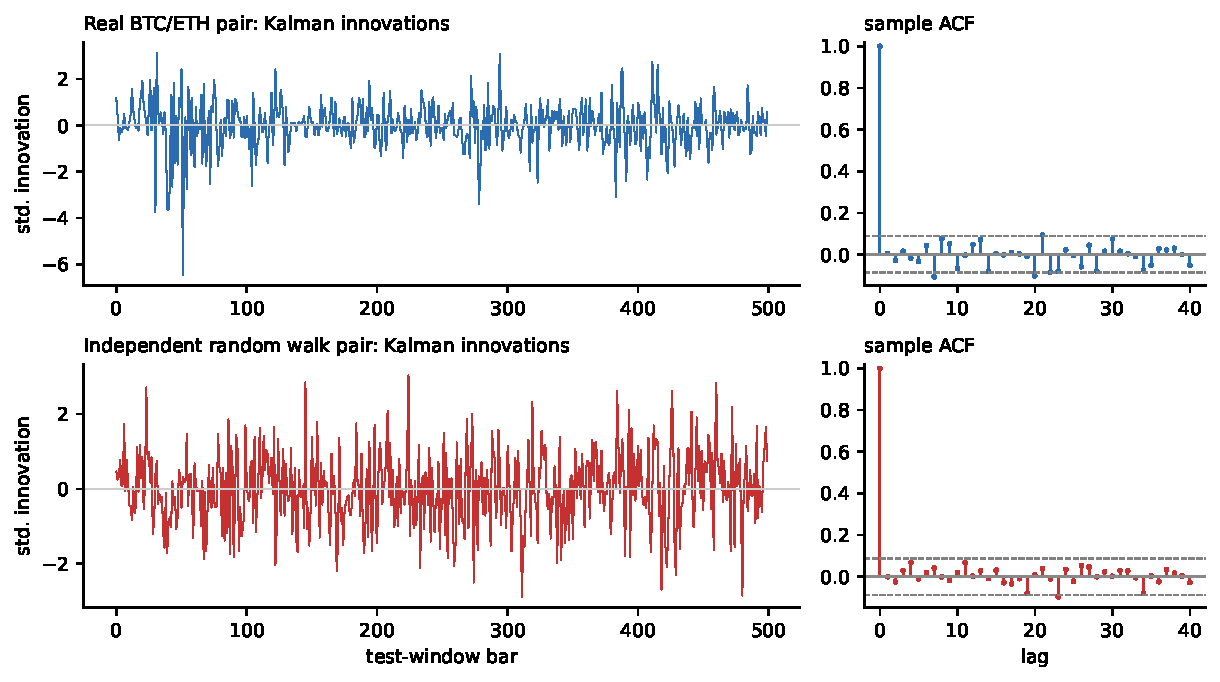
\includegraphics[width=\linewidth]{fig_kalman_innovations_white}
\caption{A Kalman filter whitens its own innovations: a representative real pair (top) and an
independent random-walk pair (bottom) produce visually indistinguishable innovation series, with
sample autocorrelation functions flat past lag $1$. This is the mechanism behind the artifact
documented in Table~\ref{tab:kalman-placebo}.}
\label{fig:kalman-innovations}
\end{figure}

\begin{table}[h]
\centering
\caption{The Kalman screen passes placebos that cannot be cointegrated at the same rate as
real pairs. Out of sample ADF on the Kalman innovations, top 50 USDT universe (250 pair
subsample), $t_0 =$
2024-01-01, 90 day train / 30 day test.}
\label{tab:kalman-placebo}
\begin{tabular}{lrr}
\toprule
Series tested & ADF $p<0.05$ & ADF $p<0.001$ \\
\midrule
Real top 50 pairs & $100.0\%$ & $96.4\%$ \\
(a) Independent random-walks & $100.0\%$ & $98.3\%$ \\
(b) Coin vs.\ phase-randomized surrogate & $100.0\%$ & $95.0\%$ \\
(c) Real pair, one leg block-shuffled & $100.0\%$ & $95.0\%$ \\
\midrule
Clean tests (EG and static OLS, test window) & $2$ to $3\%$ & n/a \\
\bottomrule
\end{tabular}
\end{table}

The artifact does not depend on that single start date. We re-ran the identical screen at
five disjoint quarterly anchors from mid-2023 to mid-2024
(Table~\ref{tab:kalman-anchors}). At every one, real pairs and all three placebos pass the
Kalman innovation ADF at $99$ to $100\%$, with Wilson $95\%$ intervals that never fall
below $95\%$, while the clean Engle-Granger benchmark stays between $1$ and $8\%$. The
screen reports the same near-total cointegration whether the input can be cointegrated or
not, at every start date we tried.

\begin{table}[h]
\centering
\caption{The artifact is not specific to one start date: the identical screen at five
disjoint quarterly anchors. Real pairs and all three placebos (independent random walk,
phase-randomized, block-shuffled) pass the Kalman innovation ADF at $p<0.05$ at nearly
$100\%$ (Wilson $95\%$ intervals in brackets; $n \approx 120$ real, $80$ per placebo),
while the clean Engle-Granger test stays low. $90$-day train / $30$-day test at each
$t_0$.}
\label{tab:kalman-anchors}
\begin{tabular}{lccr}
\toprule
Anchor $t_0$ & Real Kalman & All placebos & Clean EG \\
\midrule
2023-07-01 & $100\%$ $[97,100]$ & $100\%$ & $3.8\%$ \\
2023-10-01 & $99.2\%$ $[95,100]$ & $100\%$ & $1.4\%$ \\
2024-01-01 & $100\%$ $[97,100]$ & $100\%$ & $2.1\%$ \\
2024-04-01 & $100\%$ $[97,100]$ & $100\%$ & $8.1\%$ \\
2024-07-01 & $100\%$ $[97,100]$ & $100\%$ & $6.4\%$ \\
\bottomrule
\end{tabular}
\end{table}

We also ran a positive control: sixty constructed pairs that are genuinely cointegrated,
$y_t = x_t + e_t$ with $x_t$ a random-walk and $e_t$ a tight stationary AR(1). The Kalman screen
passes them at $100\%$, the same rate it passes the random-walk negatives, so it does not separate
true cointegration from none (Table~\ref{tab:poscontrol}). We can see the mechanism directly: the
test window innovations are white, with a Ljung-Box test failing to reject whiteness for $87\%$ of
the cointegrated pairs and $95\%$ of the random-walk pairs, while the static OLS residual stays
autocorrelated for both. The fitted hedge barely moves (median process variance
$q_\beta \approx 2\times 10^{-9}$), so the whitening comes from the filter fitting noise rather than tracking a
real relationship. The clean tests do separate the two, passing the positive control more often
than the negative ($17\%$ versus $2\%$ for Engle-Granger, $27\%$ versus $8\%$ for static OLS),
though genuine out-of-sample cointegration is hard to detect on a short window.

\begin{figure}[t]
\centering
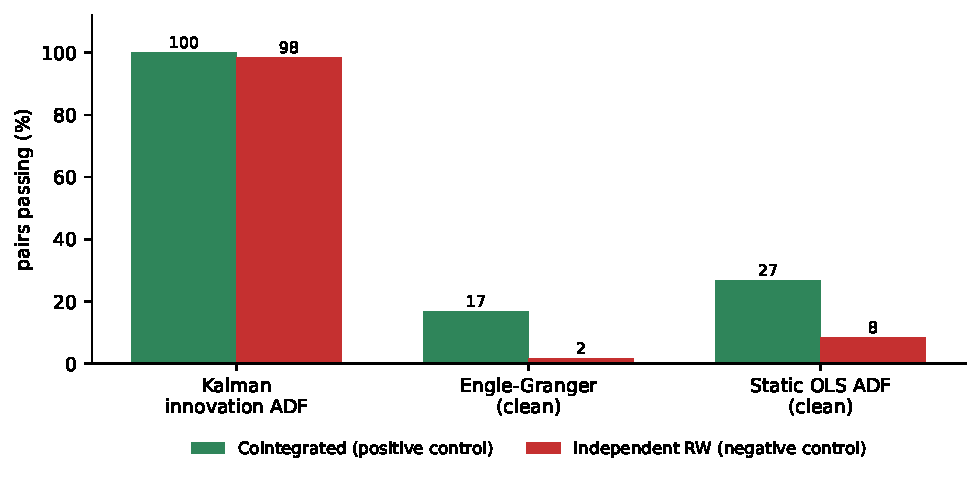
\includegraphics[width=0.82\linewidth]{fig_poscontrol_vs_negcontrol}
\caption{Positive vs negative control: the Kalman screen passes both the truly cointegrated
pairs and independent random-walks at near $100\%$, while the clean Engle-Granger and static OLS
tests separate the two groups. Visual companion to Table~\ref{tab:poscontrol}.}
\label{fig:poscontrol}
\end{figure}

\begin{table}[ht]
\centering
\caption{Positive versus negative control. The Kalman screen passes both at the same rate and its
innovations are white in both, so it does not separate them. The clean tests do. 60 constructed
pairs per group, 1500 bar train, 500 bar test.}
\label{tab:poscontrol}
\begin{tabular}{lrr}
\toprule
& Cointegrated & Random walks \\
\midrule
Kalman innovation ADF passes ($p<0.05$) & $100.0\%$ & $98.3\%$ \\
Kalman innovations white (Ljung-Box $p>0.05$) & $86.7\%$ & $95.0\%$ \\
Static OLS residual white & $0.0\%$ & $0.0\%$ \\
Clean Engle-Granger passes & $16.7\%$ & $1.7\%$ \\
Clean static OLS ADF passes & $26.7\%$ & $8.3\%$ \\
\bottomrule
\end{tabular}
\end{table}

The artifact does not depend on the bar. We reran the screen at hourly, four-hour, and daily
frequencies on a recent multiyear window (Table~\ref{tab:kalman-freq}). Real pairs and
random-walk placebos pass together at every cadence (Figure~\ref{fig:freq}): $100\%$ versus
$100\%$ versus $100\%$ at hourly and four-hour, and $70\%$ versus $68\%$ at daily ($p<0.001$). The clean tests behave differently.
Engle-Granger runs at $25\%$ on this long hourly window and falls to the $5\%$ null floor at
daily. A static OLS ADF runs higher still, from $42\%$ at hourly to $8\%$ at daily. Both are
window dependent. Over long hourly spans the crypto majors share a common trend, which a clean
test reads as broad comovement, and which the matched short window of
Table~\ref{tab:kalman-placebo} puts back at the $2$ to $3\%$ floor. Neither clean test approaches
the screen's $100\%$, and the small difference between the two tables' real $p<0.001$ rates
($96\%$ versus $100\%$) is window and sample size, not a contradiction. At the critical values
used in this pipeline, the Kalman screen does not separate real pairs from matched placebos at any
frequency we tested.

\begin{table}[h]
\centering
\caption{Frequency robustness of the Kalman artifact. Real pairs and random-walk placebos pass
the screen together at every cadence. The clean Engle-Granger and static OLS benchmarks do
not. Top-50 universe, 60 pairs per cell, recent multiyear window.}
\label{tab:kalman-freq}
\begin{tabular}{lrrrrrr}
\toprule
& \multicolumn{2}{c}{Real pairs} & \multicolumn{2}{c}{RW placebo} & \multicolumn{2}{c}{Clean tests $p<0.05$} \\
\cmidrule(lr){2-3}\cmidrule(lr){4-5}\cmidrule(lr){6-7}
Frequency & $p<0.05$ & $p<0.001$ & $p<0.05$ & $p<0.001$ & Engle-Granger & static OLS \\
\midrule
Hourly & $100.0\%$ & $100.0\%$ & $100.0\%$ & $100.0\%$ & $25.0\%$ & $41.7\%$ \\
4 hour & $100.0\%$ & $100.0\%$ & $100.0\%$ & $100.0\%$ & $11.7\%$ & $20.0\%$ \\
Daily  & $100.0\%$ & $70.0\%$  & $100.0\%$ & $68.3\%$  & $5.0\%$  & $8.3\%$ \\
\bottomrule
\end{tabular}
\end{table}

\begin{figure}[t]
\centering
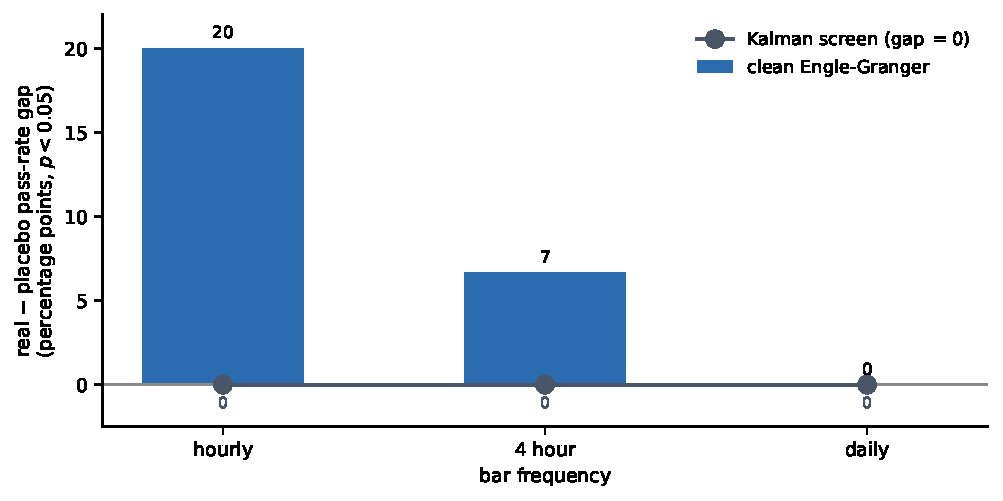
\includegraphics[width=0.74\linewidth]{fig_freq_invariance}
\caption{Placebo gap by frequency. The Kalman screen's (real minus random-walk placebo) pass rate
gap is zero to within sampling noise at every cadence, while the clean Engle-Granger test's gap is large and
frequency dependent. The clean test's random-walk placebo passes at its nominal $5\%$ size. This reshaped view makes visible what
Table~\ref{tab:kalman-freq}'s percentages only imply: a flat zero line is the diagnostic.}
\label{fig:freq}
\end{figure}

\subsection{The rolling $z$ score}
\label{sec:rollingz}

The second screen is a rolling $z$ score, the standard entry signal for pair trades. For a
spread $s_t$ it subtracts a trailing mean and divides by a trailing standard deviation,
\[
z_t = \frac{s_t - \bar{s}_{t-1}}{\sigma_{t-1}},
\]
and it trades when $|z_t|$ is large, betting the spread returns to its mean. On our spreads it
produced a large reversion edge.

The edge is mechanical. Subtracting a trailing mean from any series, including a pure random
walk, manufactures mean reversion, because the trailing mean chases the level and the deviation
from it cannot wander as freely as the raw series. Demeaning by a trailing window of length $L$
induces negative autocorrelation of order $1/L$ in the result. This is the time-aggregation
bias documented by Working~\cite{working1960correlation}: first differences of moving
averages of a random chain are spuriously correlated even when the underlying chain is not.
Cochrane~\cite{cochrane1988random}'s variance-ratio analysis of GNP gives the same lesson
from the persistence side. The floor is therefore calculable rather than fitted. A random-walk has no mean to revert to, yet
a rolling $z$ score on one still reverts.

We measured the mechanical floor two ways, and both are large. Per $|z|>2$ event, the signed
reversion on pure random-walks is positive at every frequency we tested: $+0.98z$ at hourly,
$+1.61z$ at four-hour, and $+1.51z$ at daily, each many standard deviations from zero
(Table~\ref{tab:rollingz}; Figure~\ref{fig:rollingz} shows the mechanism on one path). As a trading rule at hourly frequency, a rolling $z$ strategy that
posts a Sharpe near $4.75$ on our data still posts about $2.2$ on random-pairs and $2.4$ on
phase-randomized noise. Most of the apparent edge is the floor. For this reason every per-event
reversion magnitude elsewhere in this paper is reported net of a per-pair, per window
random-walk floor.

\begin{table}[h]
\centering
\caption{The rolling $z$ score manufactures mean reversion on pure random walks, at every
frequency. Mean signed reversion per $|z|>2$ event, 200 random-walk surrogates per cell.}
\label{tab:rollingz}
\begin{tabular}{lrr}
\toprule
Frequency & Mean event reversion ($z$) & s.d. \\
\midrule
Hourly & $+0.98$ & $0.26$ \\
4 hour & $+1.61$ & $0.39$ \\
Daily  & $+1.51$ & $0.45$ \\
\bottomrule
\end{tabular}
\end{table}

\begin{figure}[t]
\centering
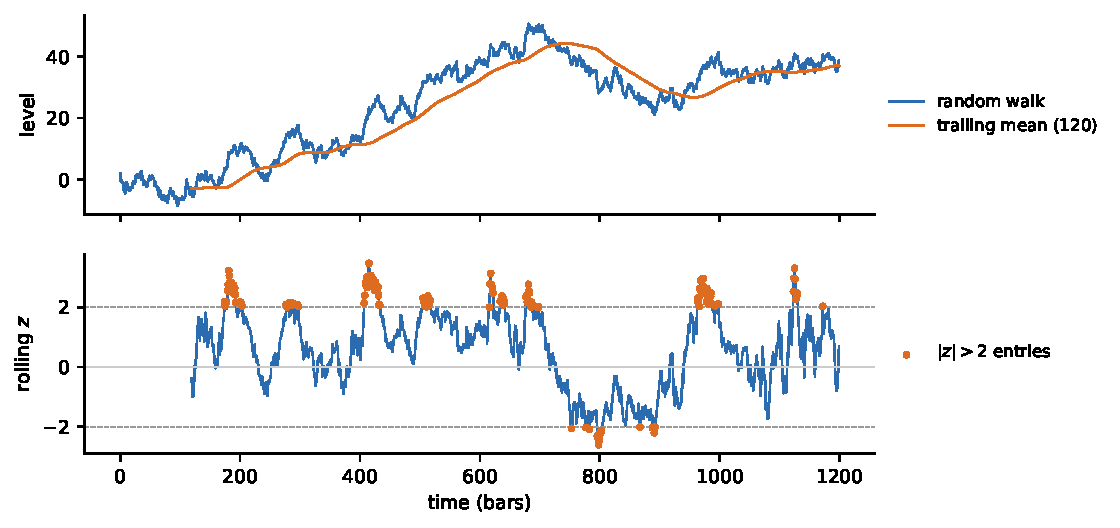
\includegraphics[width=0.78\linewidth]{fig_rollingz_noise}
\caption{A rolling $z$ score manufactures mean reversion on a pure random walk. Top: one
simulated random-walk and its trailing mean. Bottom: the resulting rolling $z$, which crosses
$\pm 2$ and reverts toward zero, although the series has no mean to revert to.}
\label{fig:rollingz}
\end{figure}

Both screens share a failure mode. They manufacture the appearance of structure that a matched
placebo reproduces. Both are robust to the analysis choices: the rolling $z$ floor stays positive
($+0.45$ to $+2.6z$) across lookback, horizon, and threshold, and the Kalman placebo passes at
$85\%$ or more across the ADF lag, so neither is an artifact of the parameters we picked. A cointegration screen built on a
filter's own innovations must be checked against a white noise placebo before it is believed,
and a rolling $z$ reversion claim must be checked against a random-walk null. Neither check is
standard practice, and without them both screens report a signal that is not there. This is the
lesson the backtest-overfitting literature draws for strategy selection~\cite{bailey2014dsr}, applied one level earlier, to
the screens that build the spread.

% =====================================================================
\section{Real but untradable structure}
\label{sec:real}

Strip the two artifacts and some genuine structure remains. None of it is tradable. Either the market prices it faster than anyone could act on it, or it is a
statistical regularity that does not turn into money. We take the clearest case of each.

\subsection{Reversion-speed persistence}

Mean reversion persists out-of-sample even though cointegration does not. Across nine disjoint
walk forward splits (six month train, three-month test), a pair's in-sample OU reversion speed (Appendix~\ref{app:ou})
predicts its out-of-sample \emph{excess} reversion, net of the rolling $z$ floor of
Section~\ref{sec:rollingz}: Spearman rank correlation $\rho = 0.46$ (95\% CI $[0.37, 0.54]$, $p<0.001$), positive
in every one of the nine splits. The top quintile shows about $0.69z$ more excess reversion than
the bottom out-of-sample ($[0.58, 0.81]$, $p<0.001$). The placebos are clean: a random
quintile split gives $+0.0001z$, and shuffling the train to test link collapses $\rho$ to
$-0.002$. Reversion speed is a real, graded, persistent property that ranks pairs.

\begin{figure}[t]
\centering
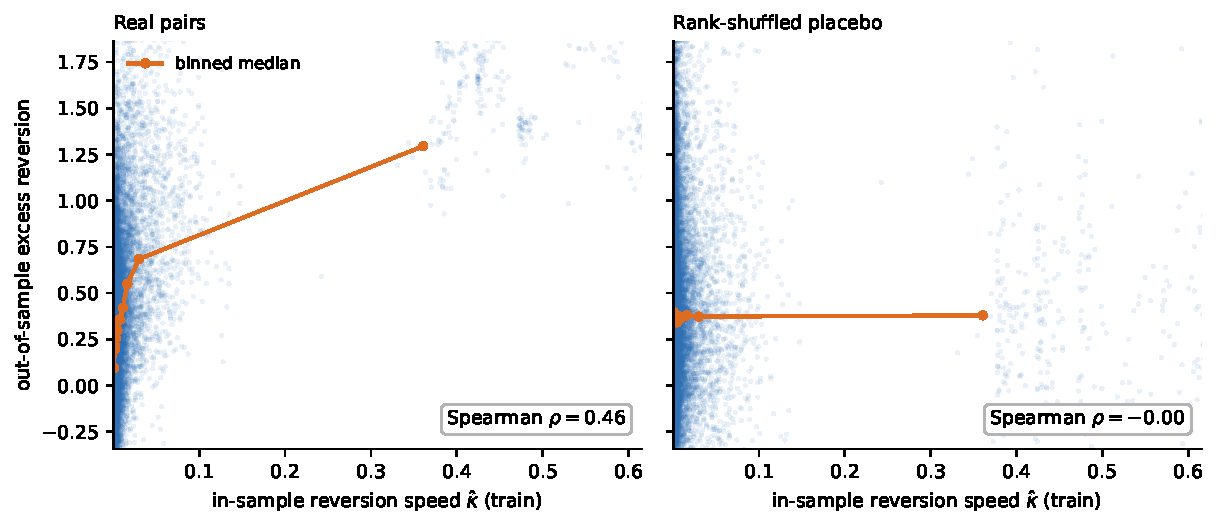
\includegraphics[width=\linewidth]{fig_reversion_persistence_scatter}
\caption{In sample OU reversion speed predicts out-of-sample excess reversion across $9$
walk forward splits (Spearman $\rho = 0.46$). Left panel: real pairs; the positive slope is
present in each of the nine splits. Right panel: rank shuffled placebo collapses to noise.}
\label{fig:rev-persist}
\end{figure}

One caveat belongs on that coefficient. The $\rho = 0.46$ is the strongest of four in-sample
reversion metrics we tried, chosen after the fact, and it is not corrected for that choice. The
direction holds across all nine splits. The exact coefficient is a best case.

Ranking pairs by reversion speed tells you where reversion lives, but not whether you can make
money on it. Extracting the edge after costs is a separate question, and the strategy built on the
property (Section~\ref{sec:survivor}) is marginal at best.

\subsection{Order flow at tradable horizons}

We tested the order flow ideas on a 2024 sample of Binance Level 2 book and trade data: aggregate
book metrics on the top 50 USDT majors, and event level tests on four majors (BTC, ETH, SOL,
AVAX) across days drawn from all twelve months, from Tardis. The book carries real,
contemporaneous information about price formation, but none of it survives to a horizon you could
trade against. That null holds for both forecasting and execution.

Trade size does proxy information. Large trades carry about twice the one second price impact of
small ones, and the ranking replicates across all of 2024 on four coins (one second impact for
BTC of $0.33/0.23/0.13$ bps for institutional, mid, and retail, with institutional $2.0$ to
$2.6\times$ retail, though the longer horizon permanent estimate is noisier;
Table~\ref{tab:institutional-impact}). Book side order flow
imbalance~\cite{contkukanovstoikov2014} explains sub-second midprice moves better than trade flow does (contemporaneous incremental $R^2$
of $+0.11$ to $+0.15$ for BTC and ETH), and $77$ to $90\%$ of the liquidity that leaves the best
quote is cancellations, invisible to trade-only analysis (Figure~\ref{fig:cancel-share}).

\begin{table}[h]
\centering
\caption{Per trade price impact at $1$-second horizon by trade size bucket and symbol: institutional
($>$\$$10$k) consistently $2.0$ to $2.6\times$ retail across BTC/ETH/SOL/AVAX, validating
size as a per-order information proxy.}
\label{tab:institutional-impact}
\begin{tabular}{lrrr}
\toprule
Symbol & Retail (bps) & Mid (bps) & Institutional (bps) \\
\midrule
BTCUSDT & $0.13$ & $0.23$ & $0.33$ \\
ETHUSDT & $0.15$ & $0.24$ & $0.32$ \\
SOLUSDT & $0.15$ & $0.26$ & $0.32$ \\
AVAXUSDT & $0.18$ & $0.38$ & $0.38$ \\
\bottomrule
\end{tabular}
\end{table}

\bigskip

\begin{figure}[t]
\centering
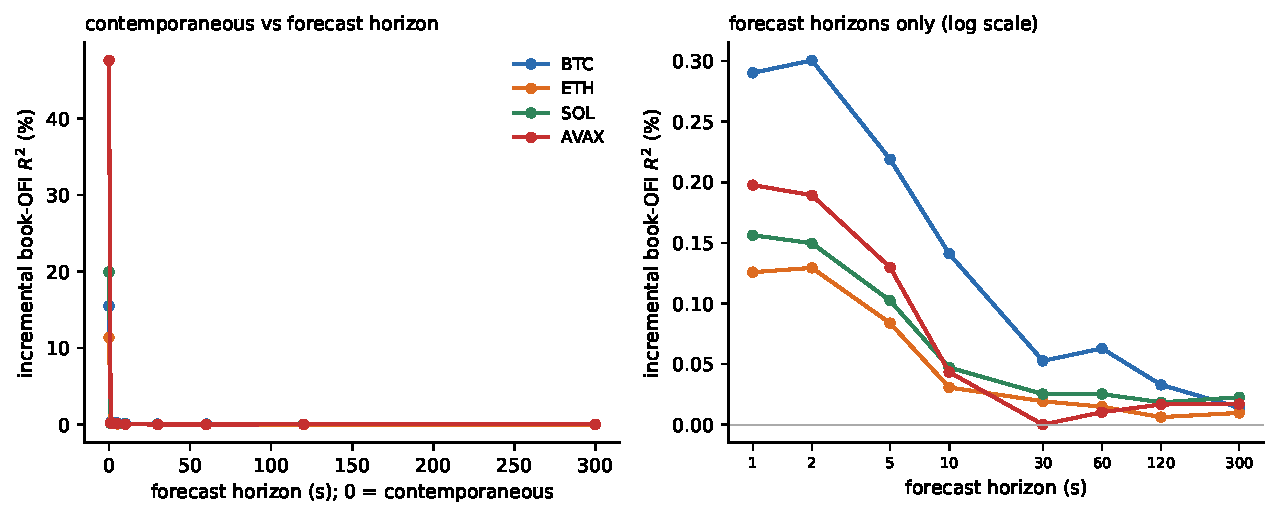
\includegraphics[width=\linewidth]{fig_ofi_decay}
\caption{Predictive incremental $R^2$ of book-OFI for forward midprice moves decays from
$\sim$$11$ to $48\%$ contemporaneously down to under $0.3\%$ at a one second forecast horizon and a $0.01$ to $0.06\%$ noise floor out to $300$ seconds, across BTC/ETH/SOL/AVAX
and all 2024 market regimes. The information half-life is seconds; no tradable forecast
horizon survives.}
\label{fig:ofi-decay}
\end{figure}

\begin{figure}[t]
\centering
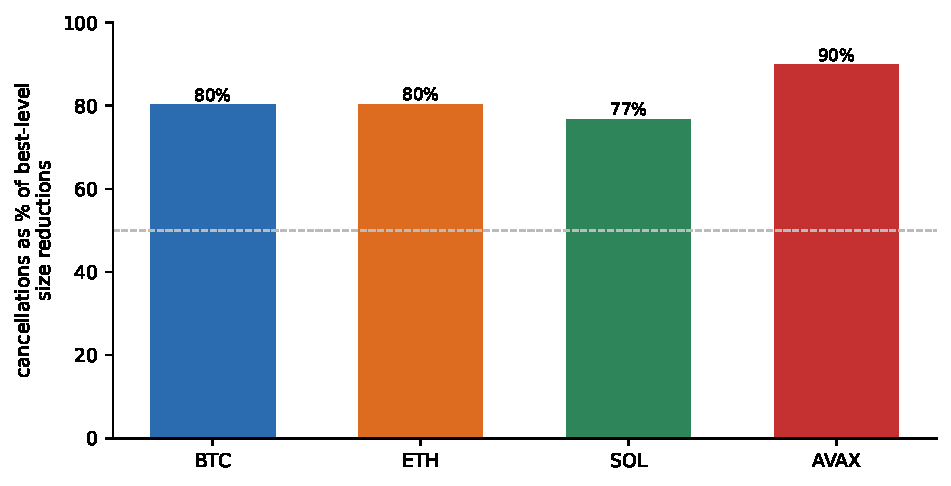
\includegraphics[width=0.66\linewidth]{fig_cancellation_share}
\caption{Cancellations dominate trades in best level liquidity withdrawal (BTC/ETH/SOL/AVAX,
2024): $77$ to $90\%$ (about $77$ to $80\%$ for BTC, ETH, SOL; $90\%$ for AVAX) of best level
size reductions are cancels, invisible to trade-only microstructure analysis. Headline figures
use a multi-day size-weighted denominator over all best-level size reductions in the sample; a
single-day strict price-equality denominator (\texttt{scratch/verify\_cancel\_share\_raw\_s3.py})
gives a lower share ($63.6\%$ BTC, $71.4\%$ ETH on 2024-03-13), and the qualitative claim that
cancels dominate trades holds under either denominator.}
\label{fig:cancel-share}
\end{figure}

All of it decays within seconds. The predictive content of order flow falls to near zero by 30
seconds (Figure~\ref{fig:ofi-decay}), and at a 15-minute to one hour horizon institutional flow predicts a mild reversal, not
continuation, with a negligible incremental $R^2$. Hidden and iceberg liquidity is measurable
(about 1 to $4\%$ of at best volume, with iceberg episode rates higher) but carries no edge.

We then measured whether the signal helps execution, the usual fallback when a signal does not
forecast returns. It does not (Table~\ref{tab:exec}). Across 29{,}952 simulated parent orders
over event level book and tape, aggressive crossing is the cheapest method for these majors, a
signal-timed passive rule does worse than a random one at the same posting rate, and the signal's
correlation with the per-order advantage of posting over crossing is $+0.03$, noise. A
perfect foresight oracle would save 1.4 bps, so the opportunity is real, but no contemporaneous book
feature forecasts it. The null holds across all twelve months of 2024, including the August 5
crash. Schnaubelt~\cite{schnaubelt2022rl} reaches the opposite headline with a different
metric and a different agent class: an RL placement policy trained on ~3.5M order book
states across 18 months posts a 37.71\% implementation-shortfall reduction vs immediate
market execution. The two findings are not in conflict. His agent learns a state-conditional
mixture of posting and crossing on a different basket and a different cost decomposition;
ours measures whether any single-shot contemporaneous L2 feature realizes the
oracle-bounded passive-vs-cross advantage on our basket. The complementarity is the
oracle bound: at 1.4 bps it caps how much any contemporaneous-feature rule on majors can
save against always-crossing, and a learned policy must work mainly through state
conditioning, not the static L2 signal. Table~\ref{tab:exec-symbol-breakdown} confirms the pooled result holds per symbol and per
order size.

\begin{table}[h]
\centering
\caption{Order flow signals do not improve execution. Implementation shortfall versus arrival
mid, pooled, 30 second horizon. Lower is cheaper. 29{,}952 orders, BTC/ETH/SOL/AVAX.}
\label{tab:exec}
\begin{tabular}{lr}
\toprule
Execution rule & Cost vs.\ arrival mid (bps) \\
\midrule
Aggressive (always cross) & $+1.10$ \\
Naive passive (always post) & $+2.69$ \\
Signal timed (post/cross on the L2 signal) & $+1.73$ \\
Random at the same posting rate & $+1.68$ \\
Oracle (perfect foresight) & $-0.30$ \\
\bottomrule
\end{tabular}
\end{table}

\begin{table}[h]
\centering
\caption{Per symbol breakdown of execution costs at \$$10$k and \$$50$k notional. Aggressive crossing
dominates across all four majors and both sizes: the L2 signal-timed rule is more expensive than crossing in every
cell, consistent with the pooled result of Table~\ref{tab:exec}.}
\label{tab:exec-symbol-breakdown}
\begin{tabular}{lrrrrr}
\toprule
& \multicolumn{2}{c}{\$$10$k notional (bps)} & \multicolumn{2}{c}{\$$50$k notional (bps)} \\
\cmidrule(lr){2-3}\cmidrule(lr){4-5}
Symbol & Aggressive & Signal timed & Aggressive & Signal timed \\
\midrule
BTCUSDT & $0.02$ & $0.64$ & $0.09$ & $0.71$ \\
ETHUSDT & $0.08$ & $0.80$ & $0.26$ & $0.94$ \\
SOLUSDT & $0.56$ & $1.36$ & $1.28$ & $2.01$ \\
AVAXUSDT & $2.09$ & $2.70$ & $4.45$ & $4.69$ \\
\bottomrule
\end{tabular}
\end{table}

The one useful byproduct is a cost number. Walking the real book puts execution costs about $17$
to $23\%$ below the flat 5 bps slippage component the earlier backtests assumed. Cheaper costs do
not rescue the strategy.

The efficiency reading is scoped to the liquid core. The Level 2 tests cover top 50 aggregate book
metrics and four megacap symbols on the global venue. The thin Binance.US microcaps where the
marginal reversion edge of Section~\ref{sec:survivor} lives are not in this sample. The two
findings plausibly fit together, though across nonoverlapping samples rather than on one venue:
the majors we can measure are efficient, and the names with an apparent edge are too thin to trade.
We did not measure the microcaps' microstructure directly, so the join is an inference.

% =====================================================================
\section{A marginal survivor}
\label{sec:survivor}

One strategy survives, but only barely. There is a real, market-neutral,
diversified mean-reversion effect in crypto pair spreads. Its tradable magnitude is uncertain, it
exists only without a stop, and a literal backtest of it inflates spectacularly. We start with the
limits, since they matter more than the headline number.

\subsection{Construction and market-neutrality}

Selecting pairs by reversion speed and holding the spread to convergence, with a static
train window hedge and $z$ score (not the rolling $z$ of Section~\ref{sec:rollingz}), produces a
positive, market-neutral return. It is diversified: beta to an equal-weight crypto index is about $-0.06$,
and the top ten principal component portfolios explain only $1.7\%$ of its return, so it is not a
hidden factor bet. It replicates on an independent exchange (Coinbase, USD quoted) and under four
from-scratch reimplementations that share none of our pipeline, none of which found look ahead,
so the effect is not a coding artifact.

\subsection{Sensitivity to the exit rule}

The exit rule decides the sign of the P\&L. With a conventional $|z| = 4$ stop the strategy loses
(Sharpe $-2.25$), and the stop is the cause: it realizes losses on spreads that then revert.
Remove the stop and hold to convergence and the strategy turns positive. The project set out to
build an hourly strategy with tight risk management. This is the opposite: a patient book that
never closes on a stop, with a median hold near 35 days, in which $78\%$ of positions do not converge within a quarter and
about a third of the return is a generic survivor comovement floor.

\subsection{Magnitude and the preregistered held-out test}

The naive Binance Sharpe was first reported near $2.5$, and four independent reimplementations put
it at $2.0$ to $2.2$. Neither is the honest figure. Month long holds make hourly returns heavily
autocorrelated (Figure~\ref{fig:hac-inflation}), so a Newey-West correction~\cite{newey1987hac}
drops the monthly Binance number to about $1.4$, and
on the independent Coinbase venue it is about $0.85$ to $0.90$. Across independent
reimplementations the Coinbase no-stop monthly Sharpe ranges $0.61$ to $0.98$ depending on entry
percentile and selection cuts; we report $0.85$ to $0.90$ as the configuration matching our
Binance specification (no-stop, $10$th-percentile entry). The HAC- and venue- honest figure
is near $1.0$ (Table~\ref{tab:venue-comparison}), and the edge concentrates in recent, high-volatility periods.

\begin{table}[h]
\centering
\caption{Naive vs HAC adjusted monthly Sharpe on
Binance.US and Coinbase for the no-stop reversion strategy. Reading: the venue gap
($\sim$$2.2$ Binance vs $\sim$$0.88$ Coinbase) and the serial correlation adjustment
(Binance naive $2.18 \to$ HAC $1.4$) together center the honest figure at $\sim$$1.0$. The
Coinbase HAC entry is not separately computed; the naive Coinbase figure is shown unchanged.}
\label{tab:venue-comparison}
\begin{tabular}{lrr}
\toprule
Series & Naive monthly Sharpe & HAC adjusted (monthly) \\
\midrule
Binance.US, hourly returns & $2.18$ & $\approx 1.4$ \\
Coinbase, hourly returns   & $0.88$ & $0.88$ \\
\midrule
HAC- and venue centered    & n/a & $\approx 1.0$ \\
\bottomrule
\end{tabular}
\end{table}

\begin{figure}[t]
\centering
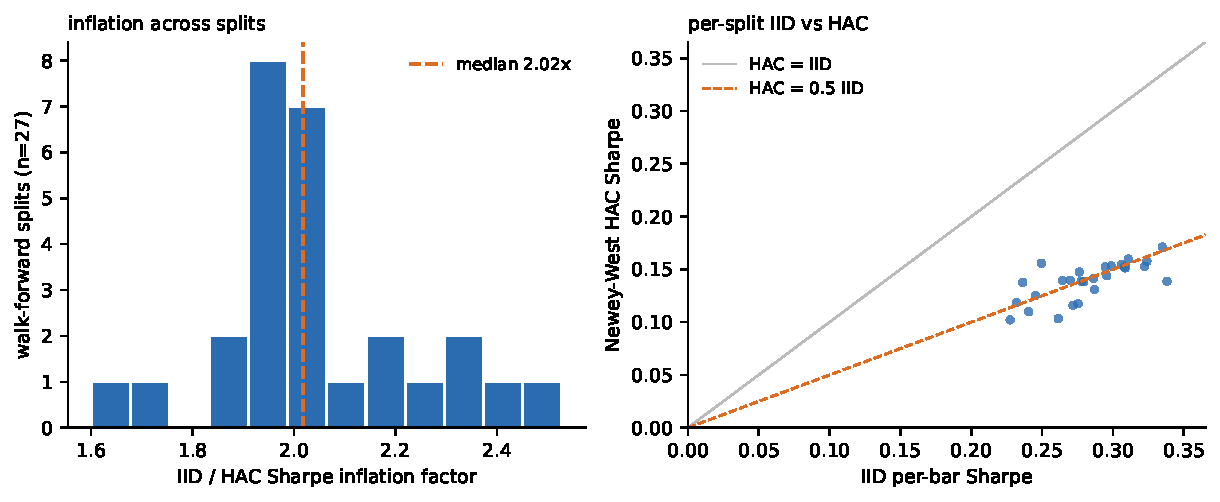
\includegraphics[width=\linewidth]{fig_hac_inflation}
\caption{Hourly Sharpe is heavily serial correlation inflated by multiweek holds. Left: per split
IID vs Newey-West HAC ratios cluster around $2\times$ (median $2.0$) across the $27$ walk forward
splits. Right: scatter of IID vs HAC Sharpe per split, with the $\mathrm{HAC} = 0.5 \cdot
\mathrm{IID}$ reference line.}
\label{fig:hac-inflation}
\end{figure}

A preregistered, held-out test makes the fragility concrete. We locked the configuration before
running (Section~\ref{sec:methods} records the lock) and evaluated it once on held-out data,
from June 2025 to May 2026. The literal result was a monthly Sharpe near $5$, \emph{higher} than the
in-sample figure, and it is not a tradable edge. It is inflation spread broadly across
high-volatility microcap alts: individual pair windows post $+300$ to $+517\%$ in three-months
under a flat 15 bps cost that badly understates the true cost of trading those names, with
unit notional accounting that ignores capacity. A $+517\%$ three-month leg implies roughly a
$150\times$ gross return, not realizable at any size. Those names are barely traded
(Figure~\ref{fig:microcap-adv}): on Binance.US
the held-out microcaps (WAXP, ZIL, VTHO, ACH, EGLD) turn over a median of tens to a few
thousand dollars a day, roughly three to four thousand times less than the majors, so the
deployable notional is negligible and a flat, size-independent cost is indefensible. The same
machinery on a venue without those microcaps returns the $\sim 1.0$ figure. So the held-out test does not confirm an alpha. It
shows the raw backtest is untrustworthy, and our own surviving result fails the same test the rest
of the paper applies to everything else.

\begin{figure}[t]
\centering
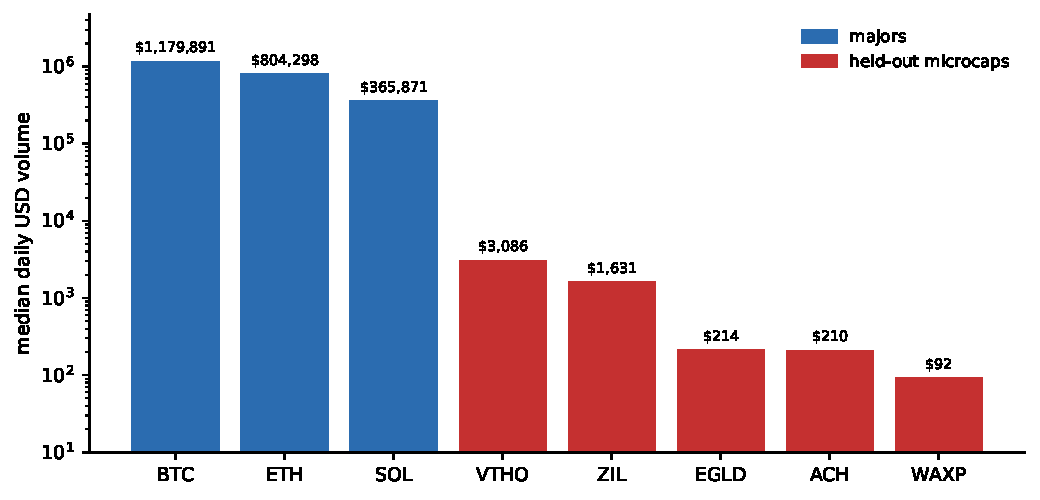
\includegraphics[width=0.82\linewidth]{fig_microcap_adv}
\caption{Median daily USD volume on Binance.US, log scale. The preregistered held-out microcaps
(WAXP, ZIL, VTHO, ACH, EGLD; red) trade at tens to a few thousand dollars per day, three to
four orders of magnitude below the majors (blue) whose costs the backtest assumes. A flat,
size-independent transaction cost is therefore indefensible on these names.}
\label{fig:microcap-adv}
\end{figure}

The preregistration had a second arm, which we report in full. A single selection over all data
before June 2025 qualified only two pairs (long-horizon reversion in the tradable band is
rare), and they posted a monthly Sharpe of $1.60$. The HAC-corrected, hourly-annualized
Sharpe on the same series is $0.95$ with $95\%$ confidence interval $[-0.21, 1.89]$, which
spans zero. The unit change (monthly vs hourly-annualized) reflects the inference: the
monthly statistic does not have enough observations on a single 11-month tail to compute a
defensible HAC interval, so the confidence statement is reported on the
hourly-annualized series where HAC at lag $240$ is well-defined. Either way, the test
confirms the inflation and gives no significant evidence for a deployable edge. The $\sim 1.0$ figure is itself exploratory, adjusted for HAC and
venue after the search, and was never preregistered.

\subsection{Conditions for deployability}

The effect is also selection sensitive and survivorship fragile. A deflated Sharpe correction
(Section~\ref{sec:methods}) survives the no-stop family of configurations but fails the whole
stop versus no-stop search, and
the supports we might cite for it (the $t$ statistic, the $\rho = 0.46$ of
Section~\ref{sec:real}, the market-neutrality) share the same universe, selection, and windows,
so they are correlated rather than independent confirmations. Its survivorship robustness rests
on the selector avoiding coins that later delist, not on surviving them: a held position in a
coin that collapses is a $-100\%$ leg. We tested this directly by forcing the book to hold through
three real collapses (LUNA, UST, FTT, each paired with BTC, with the selector's avoidance
overridden, Figure~\ref{fig:forced-collapse}). Without a stop the loss runs $-117\%$ to $-258\%$ per-pair, with intracollapse
drawdowns to $-1{,}300\%$. The structural-break circuit breaker (halt after a single leg moves more
than $50\%$ against the position) caps the loss to about $-65\%$ to $-91\%$ and the worst drawdown
to $-117\%$. The $50\%$ threshold is the tightest level at which monthly Sharpe stays within $2\%$
of the no-breaker baseline: across a sweep $K \in \{25, 30, 40, 50, 60, 70, 80, 90\}\%$,
Sharpe retention drops to $0.85$--$0.94$ for $K \le 40\%$ (the breaker fires on noise and exits
real reversion) and stays at $\sim$$1.00$--$1.02$ for $K \ge 50\%$, while the worst per-pair
loss climbs from $-131\%$ at $K = 50\%$ to $-207\%$ at $K = 90\%$. So $50\%$ is the sweet spot,
not an arbitrary cutoff. The breaker blunts the tail but does not remove it, and at the book
level it is what separates a bounded delisting risk from an unbounded one. We also inject permanent delisting scale breaks into a
fraction of the 40 pairs each quarter (Figure~\ref{fig:circuit-breaker}). Without the breaker the no-stop book's monthly Sharpe falls
to zero and then negative as the break rate rises. With the breaker it stays positive across the
whole range, keeping about $96\%$ of its monthly Sharpe at an $8\%$/yr break rate and $88\%$ at
$19\%$/yr.

\begin{figure}[t]
\centering
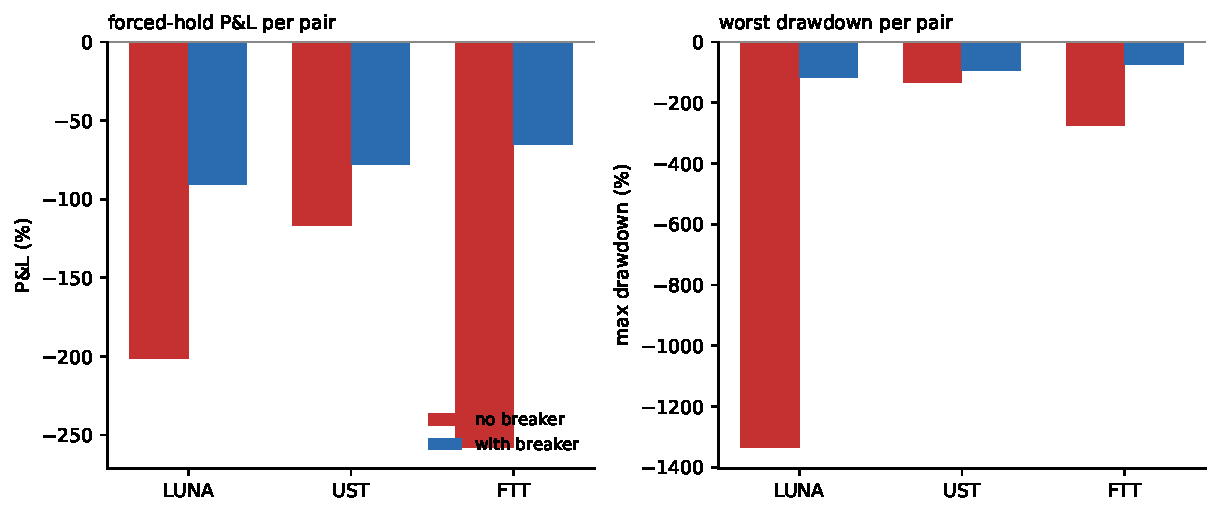
\includegraphics[width=\linewidth]{fig_forced_collapse_perpair}
\caption{Per pair P\&L when the no-stop rule is forced to hold through three real delisting
collapses (LUNA-May 2022, UST-May 2022, FTT-Nov 2022). Without the circuit breaker, losses run
$-117\%$ to $-258\%$ per-pair (a leg can lose more than $100\%$ on the log spread accounting);
with the $50\%$ single leg breaker, losses are capped at $-65\%$ to $-91\%$.}
\label{fig:forced-collapse}
\end{figure}

\begin{figure}[t]
\centering
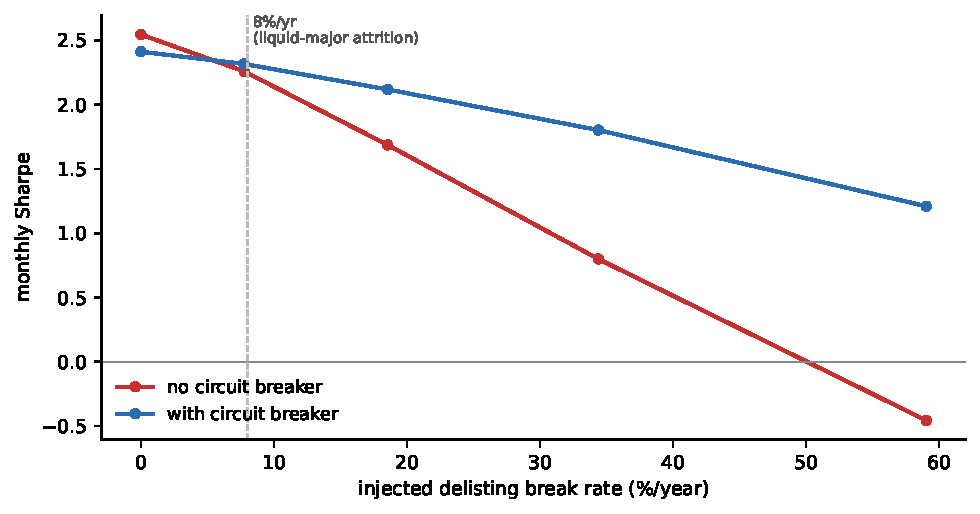
\includegraphics[width=0.8\linewidth]{fig_circuit_breaker_retention}
\caption{Monthly Sharpe of the no-stop reversion book as a function of injected delisting rate,
with and without the structural-break circuit breaker. Without the breaker, the Sharpe declines steadily and crosses zero only near a $50\%$/year
break rate. With the breaker, it retains $\approx 96\%$ of its Sharpe at the
$8\%$/year rate consistent with historical liquid major attrition.}
\label{fig:circuit-breaker}
\end{figure}

A few things make those retention figures optimistic. First, the injected breaks ramp
smoothly, so the breaker exits near its $50\%$ threshold, whereas the real gapping collapses above
cost it $-65\%$ to $-91\%$ per-pair. Second, the figures sit on the gross book, not the HAC- and
venue honest $\sim 1.0$, against which a delisting drag would bite proportionally harder. Third, the
breaks are drawn independently, which understates the way breaks cluster in market wide selloffs. The robust finding is the
qualitative one: the circuit breaker, not diversification alone, is what bounds the delisting tail,
and at the low single digit yearly attrition that liquid top 50 names actually see, the haircut is
modest. A
fully point-in-time universe of every delisted coin is still beyond our data.

The defensible claim is therefore the sensitivity itself. There is a real, market-neutral
reversion signal in crypto pair spreads that can be selected by reversion speed. Whether it is
worth anything after realistic costs, capacity, and selection is unresolved, and the most honest
single number, a monthly Sharpe near $1.0$, is an estimate that a literal backtest does not cap
from above.

% =====================================================================
\section{Limitations}
\label{sec:limits}

Five limitations bound these results, and the survivorship gap is the one most likely to change
the conclusion.

\begin{itemize}
\item \emph{Survivorship.} The local store holds currently listed symbols, so most delisted
coins are absent. The surviving strategy's robustness rests on the selector avoiding coins that
later delist. Forced to hold through three real collapses (Section~\ref{sec:survivor}) the no stop
loss runs $-117\%$ to $-258\%$ per-pair and the circuit breaker caps it near $-65\%$ to $-91\%$. A
complete point-in-time universe of every delisted coin is still beyond our data.
\item \emph{Selection.} No single configuration was fixed before the search and evaluated once
across the whole project. The preregistered test of Section~\ref{sec:survivor} covers one
configuration but cannot undo the selection that produced it, so the deflated Sharpe caution
stands.
\item \emph{Microstructure coverage.} The event-level Level 2 tests use four symbols (BTC, ETH,
SOL, AVAX) over days sampled across 2024, not a continuous year on the full universe. The
aggregate book metrics use the top 50. The execution and impact results are four symbol.
\item \emph{Single venue and quote.} The spread results are Binance.US, USDT quoted, with a
Coinbase USD-quoted cross check on the overlapping liquid majors. The microstructure is
Binance.com (global) spot. The cross-check is not a same-instrument replication: USD-quoted
Coinbase pairs have a different participant base, different fee schedule, and different
microstructure from USDT-quoted Binance.US pairs, so part of the Coinbase-Binance Sharpe
gap is venue and quote currency rather than overfitting. We have not tested other quote
currencies or a broader set of venues.
\item \emph{Costs and capacity.} Costs are a flat per-leg charge. We do not model market impact
or capacity, which is exactly what inflates the held-out microcap backtest of
Section~\ref{sec:survivor}. The corollary is that every Sharpe in the paper is a
unit-notional, capacity-unbounded figure: the no-stop reversion strategy's
$\sim$$1.0$ HAC-and-venue-corrected Sharpe is the right order of magnitude for the
qualitative claim but is not a defensible estimate of what a sized book would earn after
realistic impact. An impact-aware sized run is the constructive next step we have not done.

\item \emph{Execution-simulator fill model.} The L2 execution test of
Section~\ref{sec:real} runs $29{,}952$ simulated parent orders against the historical book,
but the fill model is intentionally simple: a posted limit order is filled when the inside
quote crosses it within the test horizon, with no queue-position tracking, no latency-to-cancel
budget, and no separate adverse-selection-conditional-on-fill treatment. This understates
the true cost of passive execution (good fills are taken first; sticky orders accumulate
adverse selection), so the negative finding for signal-timed posting is robust to making
the fill model more realistic. The perfect-foresight oracle is unaffected because it is
computed under the same fill model.
\end{itemize}

% =====================================================================
\section{Conclusion}
\label{sec:conclusion}

These negative results say more about the screens we used than about the market itself. The Kalman cointegration test and the rolling
$z$ score both pass placebos they should fail, at every frequency we tested. Order flow forecasts
only the next few seconds, a horizon no one can trade. The one market-neutral reversion effect
we find cannot be ruled out as nonexistent on the preregistered test (CI spans zero); even
our exploratory point estimate near Sharpe $1.0$ is marginal, stop sensitive, and selection
sensitive, and a literal backtest of it inflates on costs it does not model.

The lesson is a methodological habit rather than a tradable strategy. Trust a cointegration or
mean reversion screen only after you have shown it fails on a matched placebo built to reproduce
the claim if the claim is mechanical. For crypto the evidence points to microstructure efficiency in the liquid majors at
tradable horizons: the information is real, and the market has already priced it.

What would move the result is a genuinely point-in-time universe with delisted coins, a capacity and impact aware cost model, and a single preregistered configuration evaluated once on data the
search never saw. Until then, the efficiency reading holds only for the liquid core we can measure. For the thin tail,
where delisting risk concentrates, we cannot yet say.

% =====================================================================
% =====================================================================
\section*{Replication}
\label{sec:replication}

Every quantitative claim in the paper is reproducible from the public repository at
\url{https://github.com/samsam324/math-199-research}. The two screening-artifact placebos
(Section~\ref{sec:artifacts}) are in \texttt{scratch/audit\_part1.py},
\texttt{audit\_part1b.py}, and \texttt{audit\_part2.py}; the positive-control table
(Table~\ref{tab:poscontrol}) is in \texttt{scratch/kalman\_positive\_control.py}; the
$50\%$ circuit-breaker sensitivity sweep (Section~\ref{sec:survivor}) is in
\texttt{scratch/threshold\_sweep.py}; the survivorship analysis with delisted coins is in
\texttt{scratch/t2\_survivorship\_rerun.py} and \texttt{t2\_worstcase.py}; the L2 execution
test (Table~\ref{tab:exec}) is in \texttt{scratch/exec\_value\_2024.py}. The figures in
this paper were produced by \texttt{scratch/make\_figures\_v2.py}. The Level 2 dataset
(Tardis Binance.com 2024, $\sim$$175$~GB) is in S3; query helpers are in
\texttt{scripts/l2\_query.py} and a presigned-link generator is in
\texttt{scripts/presign.py}. All stochastic procedures (the $200$ random-walk surrogates,
$60$ constructed positive-control pairs, phase-randomized and block-shuffled placebos, the
$29{,}952$ simulated parent orders, block-bootstrap resamples) use fixed seeds set at the
top of each script (default \texttt{seed=42} unless documented otherwise in the script
header); rerunning a script produces the same number to the rounding precision reported in
the paper.

% =====================================================================
\begin{thebibliography}{99}

\bibitem{ammann2022survivorship}
Ammann, M., Burdorf, T., Liebi, L.~J., \& St\"ockl, S. (2022). Survivorship and delisting bias
in cryptocurrency markets. Working paper, University of St.~Gallen. SSRN~4287573.

\bibitem{andersen2014vpin}
Andersen, T.~G., \& Bondarenko, O. (2014). VPIN and the flash crash.
\emph{Journal of Financial Markets}, 17, 1--46.

\bibitem{bailey2014dsr}
Bailey, D.~H., \& L\'opez de Prado, M. (2014). The deflated Sharpe ratio: correcting for
selection bias, backtest-overfitting, and non-normality. \emph{Journal of Portfolio
Management}, 40(5), 94--107.

\bibitem{brauneis2018price}
Brauneis, A., \& Mestel, R. (2018). Price discovery of cryptocurrencies: Bitcoin and beyond.
\emph{Economics Letters}, 165, 58--61.

\bibitem{cochrane1988random}
Cochrane, J.~H. (1988). How big is the random-walk in GNP? \emph{Journal of Political
Economy}, 96(5), 893--920.

\bibitem{contkukanovstoikov2014}
Cont, R., Kukanov, A., \& Stoikov, S. (2014). The price impact of order book events.
\emph{Journal of Financial Econometrics}, 12(1), 47--88.

\bibitem{easley2012vpin}
Easley, D., L\'opez de Prado, M.~M., \& O'Hara, M. (2012). Flow toxicity and liquidity
in a high-frequency world. \emph{Review of Financial Studies}, 25(5), 1457--1493.

\bibitem{elliott2005pairs}
Elliott, R.~J., van der Hoek, J., \& Malcolm, W.~P. (2005). Pairs trading.
\emph{Quantitative Finance}, 5(3), 271--276.

\bibitem{engle1987cointegration}
Engle, R.~F., \& Granger, C.~W.~J. (1987). Co-integration and error correction:
representation, estimation, and testing. \emph{Econometrica}, 55(2), 251--276.

\bibitem{eroglu2022tvc}
Ero\u{g}lu, B.~A., Miller, J.~I., \& Yi\u{g}it, T. (2022). Time-varying cointegration and
the Kalman filter. \emph{Econometric Reviews}, 41(1), 1--21.

\bibitem{fil2020pairs}
Fil, M., \& Kristoufek, L. (2020). Pairs trading in cryptocurrency markets.
\emph{IEEE Access}, 8, 172644--172651.

\bibitem{gatev2006pairs}
Gatev, E., Goetzmann, W.~N., \& Rouwenhorst, K.~G. (2006). Pairs trading: performance of a
relative-value arbitrage rule. \emph{Review of Financial Studies}, 19(3), 797--827.

\bibitem{harvey1989structural}
Harvey, A.~C. (1989). \emph{Forecasting, Structural Time Series Models and the
Kalman Filter}. Cambridge University Press.

\bibitem{hasbrouck1991measuring}
Hasbrouck, J. (1991). Measuring the information content of stock trades.
\emph{Journal of Finance}, 46(1), 179--207.

\bibitem{krauss2017deep}
Krauss, C., Do, X.~A., \& Huck, N. (2017). Deep neural networks, gradient-boosted trees,
random forests: statistical arbitrage on the S\&P~500. \emph{European Journal of
Operational Research}, 259(2), 689--702.

\bibitem{liu2022common}
Liu, Y., Tsyvinski, A., \& Wu, X. (2022). Common risk factors in cryptocurrency.
\emph{Journal of Finance}, 77(2), 1133--1177.

\bibitem{kunsch1989block}
K\"unsch, H.~R. (1989). The jackknife and the bootstrap for general stationary
observations. \emph{Annals of Statistics}, 17(3), 1217--1241.

\bibitem{kyle1985continuous}
Kyle, A.~S. (1985). Continuous auctions and insider trading.
\emph{Econometrica}, 53(6), 1315--1335.

\bibitem{lopezdeprado2018advances}
L\'opez de Prado, M. (2018). \emph{Advances in Financial Machine Learning}. Wiley.

\bibitem{lu2021structural}
Lu, J.-Y., Lai, H.-C., Shih, W.-Y., Chen, Y.-F., Huang, S., Chang, H.-H., Wang, J.-Z.,
Huang, J.-L., \& Dai, T.-S. (2022). Structural break-aware pairs trading strategy using
deep reinforcement learning. \emph{Journal of Supercomputing}, 78(3), 3843--3882.

\bibitem{makarov2020trading}
Makarov, I., \& Schoar, A. (2020). Trading and arbitrage in cryptocurrency markets.
\emph{Journal of Financial Economics}, 135(2), 293--319.

\bibitem{newey1987hac}
Newey, W.~K., \& West, K.~D. (1987). A simple, positive semi-definite,
heteroskedasticity and autocorrelation consistent covariance matrix.
\emph{Econometrica}, 55(3), 703--708.

\bibitem{saiddickey1984}
Said, S.~E., \& Dickey, D.~A. (1984). Testing for unit roots in autoregressive-moving
average models of unknown order. \emph{Biometrika}, 71(3), 599--607.

\bibitem{schnaubelt2022rl}
Schnaubelt, M. (2022). Deep reinforcement learning for the optimal placement of cryptocurrency
limit orders. \emph{European Journal of Operational Research}, 296(3), 993--1006.

\bibitem{stoikov2018microprice}
Stoikov, S. (2018). The micro-price: a high-frequency estimator of future prices.
\emph{Quantitative Finance}, 18(12), 1959--1966.

\bibitem{triantafyllopoulos2011dynamic}
Triantafyllopoulos, K., \& Montana, G. (2011). Dynamic modeling of mean-reverting
spreads for statistical arbitrage. \emph{Computational Management Science}, 8(1--2), 23--49.

\bibitem{urquhart2016inefficiency}
Urquhart, A. (2016). The inefficiency of Bitcoin. \emph{Economics Letters}, 148, 80--82.

\bibitem{vidyamurthy2004pairs}
Vidyamurthy, G. (2004). \emph{Pairs Trading: Quantitative Methods and Analysis}.
Wiley Finance.

\bibitem{wei2018liquidity}
Wei, W.~C. (2018). Liquidity and market efficiency in cryptocurrencies.
\emph{Economics Letters}, 168, 21--24.

\bibitem{working1960correlation}
Working, H. (1960). Note on the correlation of first differences of averages in a random
chain. \emph{Econometrica}, 28(4), 916--918.

\end{thebibliography}

% =====================================================================
\appendix

\section{Methods background}
\label{sec:appendix}

This appendix collects working definitions of the tools used in the body of the paper. It
is meant for a reader who has seen probability and basic time series but may not have used
all of these specific instruments. We keep proofs out and give the formulas that are
actually invoked in the text. Section references in parentheses point to where the tool is
used.

\subsection{Kalman filter and state-space form for dynamic hedge ratios}
\label{app:kalman}

Let $y_t$ be the dependent log price and $x_t$ the independent log price in a pair. The
dynamic hedge model treats the intercept $\alpha_t$ and slope $\beta_t$ as latent states
that drift over time. The state-space form is
\[
\theta_t \;=\; \theta_{t-1} + w_t, \qquad w_t \sim \mathcal{N}(0, Q),
\]
\[
y_t \;=\; H_t \, \theta_t + v_t, \qquad v_t \sim \mathcal{N}(0, R),
\]
with $\theta_t = (\alpha_t, \beta_t)^\top$, observation matrix $H_t = (1, x_t)$, state-noise
covariance $Q \in \mathbb{R}^{2\times 2}$, and observation-noise variance $R > 0$. The
states follow a random walk; only $y_t$ is observed.

Given the prior state mean $\hat{\theta}_{t-1|t-1}$ and covariance $P_{t-1|t-1}$, the
Kalman recursion predicts
\[
\hat{\theta}_{t|t-1} = \hat{\theta}_{t-1|t-1}, \qquad P_{t|t-1} = P_{t-1|t-1} + Q,
\]
forms the one-step innovation
\[
e_t \;=\; y_t - H_t \hat{\theta}_{t|t-1}, \qquad S_t \;=\; H_t P_{t|t-1} H_t^\top + R,
\]
computes the Kalman gain
\[
K_t \;=\; P_{t|t-1} H_t^\top S_t^{-1},
\]
and updates
\[
\hat{\theta}_{t|t} = \hat{\theta}_{t|t-1} + K_t e_t, \qquad P_{t|t} = (I - K_t H_t) P_{t|t-1}.
\]
The gain $K_t$ is the optimal blend of model prediction and new observation. The
hyperparameters $Q$ and $R$ are estimated by maximizing the Gaussian innovation likelihood
\[
\log \mathcal{L}(Q, R) \;=\; -\tfrac{1}{2} \sum_{t} \left( \log 2\pi S_t + e_t^2 / S_t \right),
\]
on a training window, then frozen and forward-rolled on the test window so no test-window
information leaks into the filter.

The mechanism behind the artifact in Section~\ref{sec:kalman} lives in the innovation
sequence. By construction, $\{e_t / \sqrt{S_t}\}$ has zero mean, unit variance, and zero
serial correlation under the model, and at steady state the filter approaches this
whitening behavior for any input~\cite{harvey1989structural}. Running a stationarity test
on $e_t$ therefore measures how well the filter has been optimized, not whether $y_t$ and
$x_t$ share a common stochastic trend. A test that rejects the unit root on $e_t$ is
consistent with no cointegration whatsoever.

\subsection{Augmented Dickey-Fuller test}
\label{app:adf}

The augmented Dickey-Fuller (ADF) test of Said and Dickey~\cite{saiddickey1984} tests the
null $H_0$: the series $z_t$ has a unit root (is $I(1)$) against $H_1$: $z_t$ is
stationary. The test regression is
\[
\Delta z_t \;=\; \mu + \rho \, z_{t-1} + \sum_{i=1}^{p} \gamma_i \, \Delta z_{t-i} + \varepsilon_t,
\]
with the augmentation lags included to soak up short-run serial correlation in
$\varepsilon_t$. The test statistic is the $t$-ratio on $\hat{\rho}$, compared against
Dickey-Fuller critical values. Under $H_0$, $\rho = 0$ and the process is a random walk;
under $H_1$, $\rho < 0$ and shocks decay geometrically. Reject for sufficiently negative
$t_{\hat\rho}$.

The connection to the Kalman innovation artifact (Section~\ref{sec:kalman}) is mechanical: a
series that is close to white noise has trivially fast mean reversion, so the ADF rejects
easily even when no economic mean-reverting relation is present. The test answers ``is this
stationary'', not ``is this a cointegrating residual''.

\subsection{Engle-Granger cointegration}
\label{app:eg}

Two integrated series $y_t, x_t \sim I(1)$ are cointegrated if there exists a constant
$\beta$ such that $y_t - \beta x_t$ is $I(0)$. The Engle-Granger two-step
procedure~\cite{engle1987cointegration} fits this $\beta$ by static OLS on levels,
\[
y_t \;=\; \alpha + \beta x_t + u_t,
\]
forms the residuals $\hat{u}_t = y_t - \hat\alpha - \hat\beta x_t$, and applies an ADF test
to $\hat{u}_t$ with Engle-Granger critical values (which are more conservative than ADF
because $\hat\beta$ has been estimated). Rejection is evidence that the linear combination
defined by $(\hat\alpha, \hat\beta)$ is a stationary error-correction term.

This is the clean comparison for the Kalman-innovations procedure of
Section~\ref{app:kalman}. Engle-Granger tests a residual whose dynamics are inherited from
the original prices; the Kalman procedure tests an innovation sequence whose dynamics are
inherited from the filter. The latter rejects the unit root on placebos that, by
construction, cannot be cointegrated; the former does not.

\subsection{Newey-West HAC standard errors}
\label{app:hac}

Ordinary OLS standard errors assume the regression errors are independent and
homoskedastic. In time series with overlapping returns, slow-moving regressors, or
autocorrelated targets, both assumptions fail and naive standard errors understate sampling
uncertainty, often by a large factor. The HAC covariance estimator of
Newey and West~\cite{newey1987hac} corrects this. For a regression with score $g_t$, the
Newey-West variance estimator is
\[
\hat{\Sigma}_{NW} \;=\; \hat{\Gamma}_0 + \sum_{\ell = 1}^{L} w_\ell \, \big( \hat{\Gamma}_\ell + \hat{\Gamma}_\ell^\top \big),
\qquad
w_\ell \;=\; 1 - \frac{\ell}{L+1},
\]
where $\hat{\Gamma}_\ell = T^{-1} \sum_{t = \ell+1}^{T} g_t g_{t-\ell}^\top$ is the sample
autocovariance at lag $\ell$ and $w_\ell$ is the Bartlett kernel. The kernel is
non-negative and linearly decreasing in $\ell$, which guarantees a positive semi-definite
estimate.

We use $L = 60$ for one-hour analyses with a 60-bar target, $L = 24$ for daily analyses
with a one-day target, and $L = 240$ for monthly Sharpe inference where ten daily lags
buffer the monthly aggregation. Sharpe ratios reported as ``HAC adjusted'' divide the mean
by the square root of the HAC variance of the mean, then scale to monthly.

\subsection{Deflated Sharpe Ratio}
\label{app:dsr}

The deflated Sharpe ratio (DSR) of Bailey and L\'opez de Prado~\cite{bailey2014dsr}
discounts a reported Sharpe for non-normal returns and for the number of strategies that
were tried before the one that was reported. Let $\widehat{SR}$ be the in-sample Sharpe of
the selected strategy, $T$ the sample length, $\gamma$ the sample skewness, and $\kappa$
the sample kurtosis. The DSR is
\[
\mathrm{DSR} \;=\; \Phi\!\left( \frac{ (\widehat{SR} - SR_0) \, \sqrt{T - 1} }
    { \sqrt{1 - \gamma \, \widehat{SR} + \tfrac{\kappa - 1}{4} \, \widehat{SR}^{\,2} } } \right),
\]
where $\Phi$ is the standard normal CDF. The threshold $SR_0$ is the expected maximum
Sharpe under the null of zero true edge across $N$ independent trials,
\[
SR_0 \;=\; \sqrt{V[\,\widehat{SR}_n\,]} \left( (1 - \gamma_E) \, \Phi^{-1}\!\big(1 - 1/N\big)
    + \gamma_E \, \Phi^{-1}\!\big(1 - 1/(N e)\big) \right),
\]
with $\gamma_E \approx 0.5772$ the Euler-Mascheroni constant and $V[\widehat{SR}_n]$ the
cross-trial variance of estimated Sharpes under the null.

$N$ matters because the maximum of $N$ noisy estimates grows with $N$: trying ten
strategies and reporting the best one has a much higher null Sharpe than trying one.
Doubling the number of trials raises $SR_0$ by roughly $\sqrt{\log N}$ in the relevant
regime. We use $N$ equal to the number of distinct parameter or pair configurations
evaluated before the reported one.

\subsection{Ornstein-Uhlenbeck process and reversion speed}
\label{app:ou}

The Ornstein-Uhlenbeck (OU) process is the canonical continuous-time mean-reverting model.
The SDE is
\[
dS_t \;=\; \kappa \, (\mu - S_t) \, dt + \sigma \, dW_t,
\]
with long-run mean $\mu$, reversion speed $\kappa > 0$, instantaneous volatility $\sigma$,
and $W_t$ a Wiener process. The conditional mean decays geometrically toward $\mu$ with
rate $\kappa$, so the expected time for a deviation to halve is the half-life
\[
t_{1/2} \;=\; \frac{\ln 2}{\kappa}.
\]
We estimate $\kappa$ from a discretized AR(1) fit on the spread,
$S_{t+1} - S_t = a + b (S_t - \mu) + \eta_t$ with $\hat{\kappa} = -\ln(1 + b) / \Delta t$,
and rank pairs by this estimate.

The finding in Section~\ref{sec:real} that train-window $\hat\kappa$ predicts test-window
$\hat\kappa$ at Spearman $\rho = 0.46$ across walk-forward splits is a statement about the
process, not about profitability.

\subsection{Walk-forward cross-validation}
\label{app:wf}

Walk-forward cross-validation is the non-anticipative analogue of $k$-fold CV for time
series. Fix a train length $T_{\mathrm{tr}}$, a test length $T_{\mathrm{te}}$, and a step
length $T_s$. Split $i$ uses observations $[t_i, t_i + T_{\mathrm{tr}})$ for fitting and
$[t_i + T_{\mathrm{tr}}, t_i + T_{\mathrm{tr}} + T_{\mathrm{te}})$ for evaluation, then
advances $t_{i+1} = t_i + T_s$. Any parameter is refit per split using only the train
window. Results are reported as the distribution across splits, not as a single in-sample
number.

We use $T_{\mathrm{tr}} = 6$ months, $T_{\mathrm{te}} = 3$ months, and $T_s = 3$ months in
most of the paper, with $90/30$ in earlier microstructure work. Random $k$-fold is
inappropriate for time series because it routinely places train observations after test
observations and destroys the no-lookahead guarantee.

\subsection{Placebo construction}
\label{app:placebo}

A placebo is a synthetic series with a known absence of the structure being tested.
Different nulls preserve different features, and the right placebo is the one that matches
everything in the data except the mechanism in question. We use four.

\emph{Random walks via cumulative sums.} Sample $\eta_t \sim \mathcal{N}(0, \sigma^2)$
i.i.d.~and set $z_t = z_{t-1} + \eta_t$. This preserves nothing about the original series
except the innovation variance; two independent random-walks share no common trend.

\emph{Phase randomization.} Take the discrete Fourier transform $\tilde{z}_k =
\mathcal{F}[z_t]$, replace each non-DC phase by a uniform draw on $[0, 2\pi)$ subject to
Hermitian symmetry, and invert. The resulting series has the same power spectrum as the
original but random phase, so all linear second-order statistics are preserved while any
non-linear or cross-series alignment is destroyed.

\emph{Block shuffle.} Partition $z_t$ into contiguous blocks of length $L$ and concatenate
the blocks in a random order. Short-range autocorrelation up to lag $\sim L$ is preserved;
long-range structure including unit roots and cointegrating drift is destroyed.

\emph{Random-pair pairing.} Keep each price series intact but pair it with the price series
of an unrelated coin. Marginal distributions, autocorrelations, volatility clustering, and
trends are all preserved leg by leg; only the joint cointegration is destroyed.

The four nulls answer different questions. The Kalman screen of Section~\ref{sec:kalman}
fails the random-walk, phase-randomized, and block-shuffled nulls at the same rate as the real data,
which is the diagnostic.

\subsection{Microstructure terms}
\label{app:micro}

\emph{Mid quote.} $p^{\mathrm{mid}}_t = (p^a_t + p^b_t)/2$, with $p^a_t$ the best ask and
$p^b_t$ the best bid.

\emph{Quoted spread.} $s_t = p^a_t - p^b_t$. The relative spread is $s_t /
p^{\mathrm{mid}}_t$.

\emph{Microprice.} The size-weighted mid of Stoikov~\cite{stoikov2018microprice},
\[
p^{\mathrm{micro}}_t \;=\; \frac{q^b_t \, p^a_t + q^a_t \, p^b_t}{q^a_t + q^b_t},
\]
with $q^a_t, q^b_t$ the displayed sizes at the top of book. The microprice tilts toward the
side with less depth.

\emph{Order book imbalance.} For top $K$ levels,
\[
\mathrm{OBI}_t^{(K)} \;=\; \frac{\sum_{k=1}^{K} q^b_{t,k} - \sum_{k=1}^{K} q^a_{t,k}}
    {\sum_{k=1}^{K} q^b_{t,k} + \sum_{k=1}^{K} q^a_{t,k}} \;\in\; [-1, 1].
\]

\emph{Order flow imbalance.} The best-level event-time OFI of Cont, Kukanov, and
Stoikov~\cite{contkukanovstoikov2014} is built from changes in displayed depth at the inside,
\[
e_t \;=\; \mathbb{1}\{p^b_t \geq p^b_{t-1}\} q^b_t - \mathbb{1}\{p^b_t \leq p^b_{t-1}\} q^b_{t-1}
    - \mathbb{1}\{p^a_t \leq p^a_{t-1}\} q^a_t + \mathbb{1}\{p^a_t \geq p^a_{t-1}\} q^a_{t-1},
\]
and the aggregated OFI over a window is
$\mathrm{OFI}_{[\tau_1, \tau_2]} = \sum_{t: \tau_1 \leq t < \tau_2} e_t$.

\emph{VPIN.} The volume-synchronized probability of informed trading of Easley, L\'opez de
Prado, and O'Hara~\cite{easley2012vpin} groups trades into equal-volume buckets of size $V$
and computes, within bucket $j$,
\[
\mathrm{VPIN}_j \;=\; \frac{1}{n} \sum_{i=j-n+1}^{j} \frac{|V_i^B - V_i^S|}{V},
\]
with $V_i^B$ and $V_i^S$ the buy- and sell-classified volume in bucket $i$ and $n$ the
window length in buckets.

\emph{Permanent vs transient impact.} Hasbrouck~\cite{hasbrouck1991measuring} decomposes
the mid-quote response to a trade into a permanent component (information) that persists in
the efficient price and a transient component (liquidity) that decays as inventory works
off.

\subsection{Block bootstrap}
\label{app:bb}

The i.i.d.~bootstrap is invalid for autocorrelated series because it destroys the serial
structure that drives sampling uncertainty. The block bootstrap of
K\"unsch~\cite{kunsch1989block} preserves it. From a series $\{z_t\}_{t=1}^{T}$, draw
$\lceil T / L \rceil$ blocks of length $L$ with replacement, where each block is a
contiguous slice $(z_s, z_{s+1}, \dots, z_{s+L-1})$ with $s$ uniform on
$\{1, \dots, T\}$ with indices taken modulo $T$ (the circular block bootstrap we use), concatenate them, and truncate to length $T$. Resample $B$ times
to form the bootstrap distribution.

The block length $L$ governs the bias-variance trade-off: $L$ must be large enough that
adjacent blocks are approximately independent, but small enough that enough distinct blocks
exist. We use $L = 300$ for hourly series, roughly twelve trading days.

\end{document}
